\section{HO SiPM Upgrade}
\begin{itemize}
\item(Was there an introduction to HO already? If no, this goes here...)
\end{itemize}
In the first long shutdown of the LHC, the Outer Hadron Calorimeter (HO) was subject to upgrades. The previously used HPDs\footnote{{\bf H}ybrid {\bf P}hoto-{\bf D}iodes} were replaced by SiPMs\footnote{{\bf Si}licon {\bf P}hoto-{\bf M}ultipliers} due to bad performance. The SiPM readout was designed as a drop-in replacement to keep most of the readout chain. The SiPMs were arranged on a newly produced PCB\footnote{{\bf P}rinted {\bf C}ircuit {\bf B}oard} to match the position of the pixels of the HPDs. The arrangement of the SiPMs is shown in Fig. \ref{sipmPcb}.
\begin{figure}[h]
\centering
\begin{minipage}[t]{0.475\textwidth}
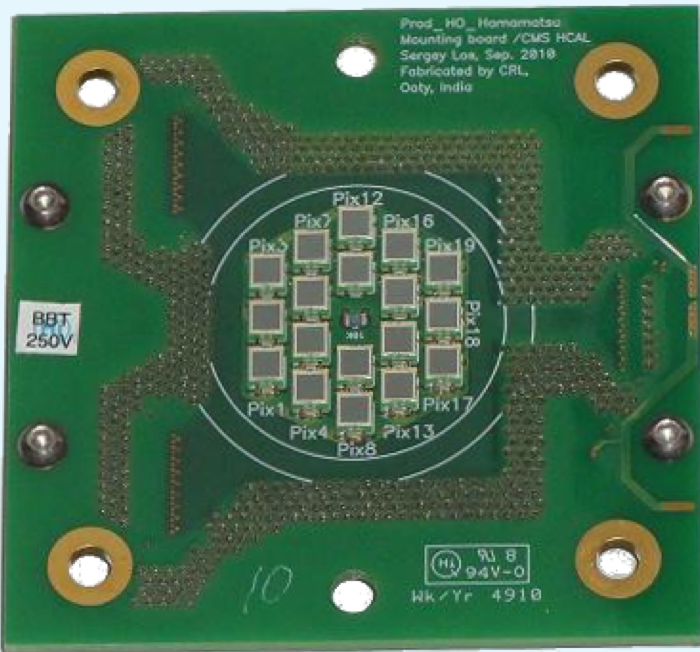
\includegraphics[width=\textwidth]{Bilder/pcbSipm.png}
\caption{PCB carrying 18 SiPMs. The white cirlce marks the position of the removed HPDs.}
\label{sipmPcb}
\end{minipage}
\hspace{1cm}
\begin{minipage}[t]{0.435\textwidth}
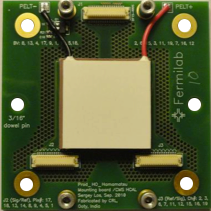
\includegraphics[width=\textwidth]{Bilder/pcbPeltier.png}
\caption{Backside of an HO PCB with the Peltier element attached.}
\label{peltier}
\end{minipage}
\end{figure}
It can be seen that the new PCB has 18 SiPMs in the position where the 18 pixels of the HPDs were.
The installed SiPM type was produced by Hamamatsu and is identical to a Hamamatsu S10931-050. It has an area of (3x3) mm$^2$ and comes with an SMD type housing. The cell pitch is 50 $\mu$m. A key feature of the device is the change of the breakdown voltage with respect to the temperature. The manufacturer specifies this quantity to be 56 $\frac{\text{mV}}{\text{K}}$.
Because HO has two layers of scintillator in ring 0, whereas rings $\pm$1 and $\pm$2 have only one layer of scintillator, the number of fibers arriving at a single SiPM is larger in ring 0. As a consequence, the fibers cannot be arranged such that they completely fit inside the area of an SiPM. Therefore, a light mixer is installed between the ends of the fibers and the SiPM surface in ring 0. This light mixer distributes the light of the fibers uniformly over an SiPM's surface and compensates for light losses at the edges of an SiPM.
With SiPMs being solid state devices and thus being rather sensitive to temperature changes it is inevitable to provide a controlled temperature environment for a stable operation of the devices. For this reason the PCBs carrying the SiPMs are equipped with Peltier elements on their backsides. Fig. \ref{peltier} shows a mounted Peltier element on a PCB.
\subsection{System Performance}
\subsubsection{Temperature}
The features of an SiPM may change strongly with the temperature if not corrected for. For this reason it is important to control the temperature of an SiPM before studying other parameters to be sure that any observed change is not due to a change in the temperature. Fig. \ref{temperatureStability} shows  temperature deviations from a reference temperature plotted vs. time for a single carrier PCB.
\begin{figure}[h]
\centering
\begin{minipage}[t]{0.475\textwidth}
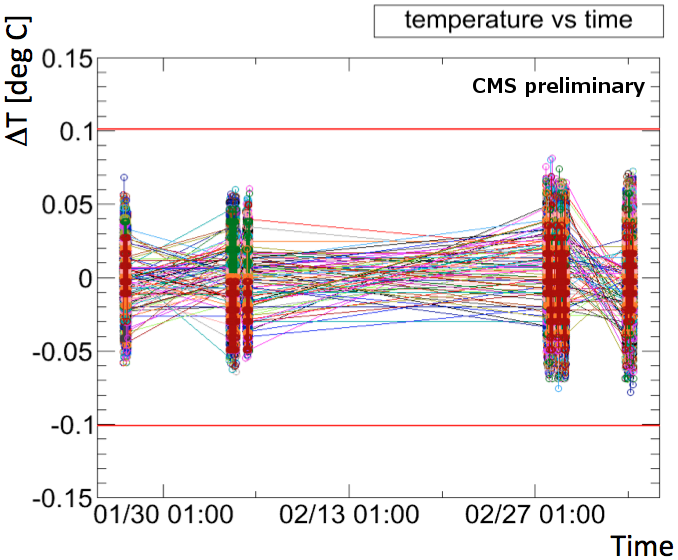
\includegraphics[width=\textwidth]{Bilder/temperature.png}
\caption{Fluctuation of temperature at a PCB plotted against time. The fluctuations stay within 0.1 $^\circ$C.}
\label{temperatureStability}
\end{minipage}
\hspace{0.5cm}
\begin{minipage}[t]{0.455\textwidth}
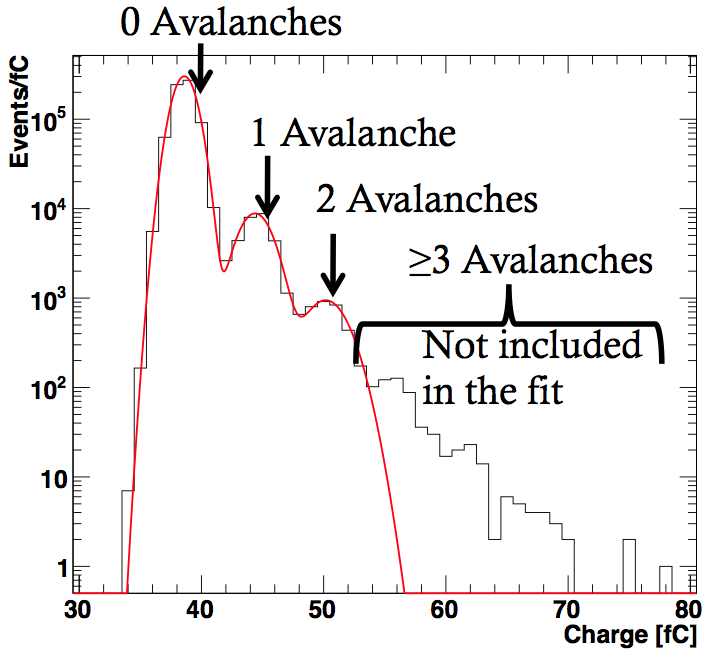
\includegraphics[width=\textwidth]{Bilder/gainDetermination.png}
\caption{Dark noise spectrum of an SiPM. plotted in red is the fit that is used for gain determination.}
\label{darkNoise}
\end{minipage}
\end{figure}
It is evident that the deviations stay within a range of 0.1 $^\circ$C which corresponds to a change of 5.6 mV in the bias voltage

\subsubsection{Gain}
The gain determines the signal height that is produced by an SiPM and thus the measured charge in data taking. Hence, it is necessary to know the gain of an SiPM to be able to tell the number of photons that triggered the SiPM and get a measure of the deposited energy in the detector. HO uses two ways of determining the gain.
The first is to use the dark noise spectrum of an SiPM that develops due to thermal exication of electrons in the active volume of an SiPM cell and the subsequent breakdown ot that cell. A gauss fit is performed to the pedestal peak and the peaks of one and two avalanches and from the distance of the peak positions the gain is calculated. An example dark noise spectrum together with an applied fit is shown in Fig. \ref{darkNoise}.
\begin{figure}[h]
\centering
\begin{minipage}[t]{0.475\textwidth}
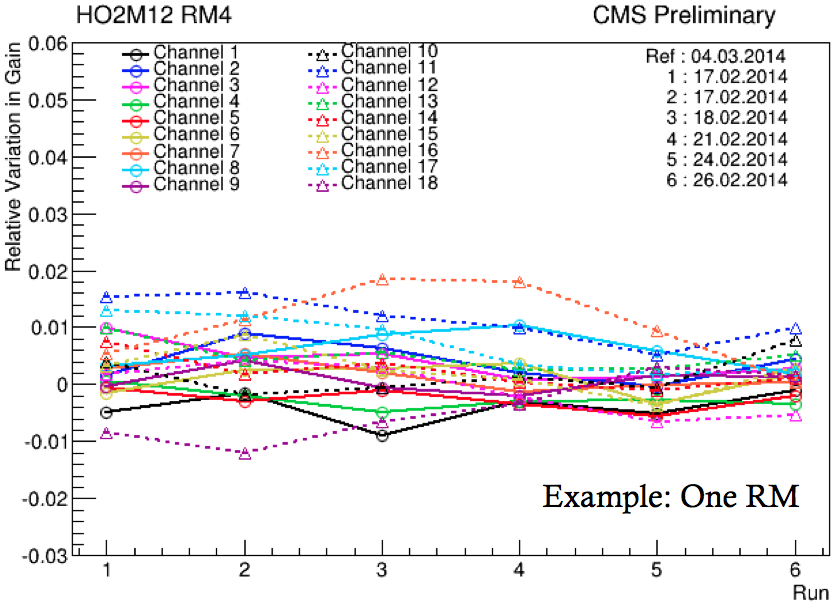
\includegraphics[width=\textwidth]{Bilder/gainOverTime.png}
\caption{Relative gain variation against time using the dark noise spectrum for gain determination.}
\label{gainVsTime}
\end{minipage}
\hspace{0.5cm}
\begin{minipage}[t]{0.475\textwidth}
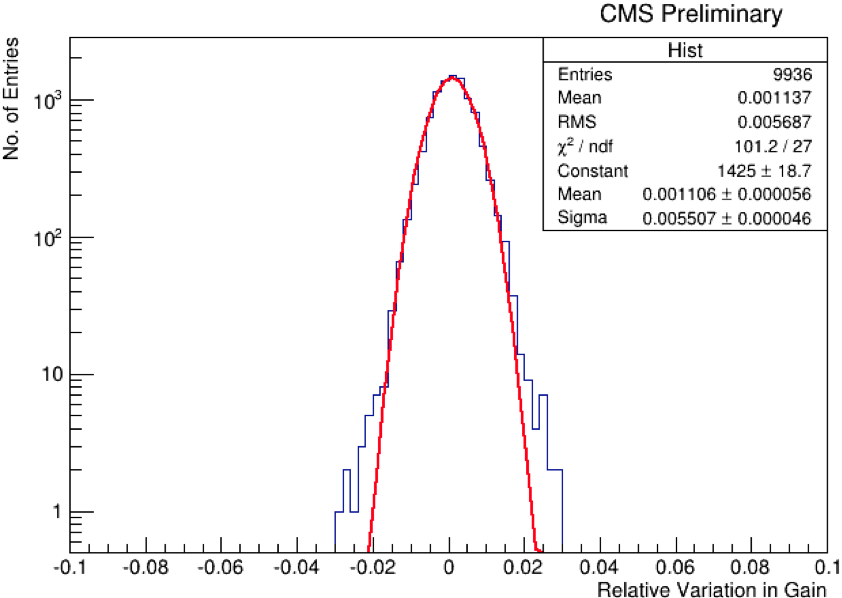
\includegraphics[width=\textwidth]{Bilder/gainTotal.png}
\caption{Histogram of all measured relative gain variations using the dark noise spectrum. The measurements were performed during the same period as is shown in Fig. \ref{gainVsTime}.}
\label{gainHist}
\end{minipage}
\end{figure}
The second method uses short light pulses from an LED that are led onto the SiPMs. When the light pulses contain not too many photons, the resulting signal distribution has a mean of N$\times$gain and a width of $\sqrt{\text{N}}\times$gain, assuming Poisson statistics for the uncertainty of the number of photons. Dividing the square of the measured width of the distribution by the measured mean, one obtains the gain of an SiPM.
Before reviewing the comparability of the different methods it is necessesary to assure that the means of gain determination are stable in themselves with respect to time. The relative gain variation against time using the dark nosie spectrum is depicted in Fig. \ref{gainVsTime}. It can be found that for a single PCB the relative gain variation stays within a 2 \% frame. A histogram showing the relative gain variations for the same period for all installed SiPMs is plotted in Fig. \ref{gainHist}. The largest variations can be found to be within 3 \%. Having shown that the gain determination yields stable results, it is worthwhile to examine the correlation between the two ways of determining the gain. The result of a correlation plot is printed in Fig. \ref{gainCorr}. The plot shoes that the measured gain values are centralized around a specific value and no large deviation are found. However, it can be noticed that the mean gain value for the LED method is systematically shifted with respect to the results from the dark noise spectrum. This shift can be explained by the fact that the spectrum measured with the LED method is not exactly gaussian. This results in a shift towards higher gain values for this method. Once this offset has been characterized it would be possible to correct for it.

\subsubsection{Breakdown Voltage}
The gain of an SiPM depends on the voltage difference between the applied voltage and the breakdown voltage of the device. It is therefore necessary to have reliable means of determining the breakdown voltage of an SiPM in order to keep the gain stable. In HO there are two ways of measuring the breakdown voltage. The first one exploits again the dark noise spectrum of an SiPM. By measuring the gain with the dark noise spectrum for different bias voltages one may plot the gain versus the bias voltage. By fitting a straight line to the distribution and extrapolate to a gain of zero the breakdown voltage is found. The second way of gain determination uses an LED again. The collected charge is measured for different bias voltages and then the relative derivative $\frac{\text{dS}}{\text{SdV}}$ is calculated. The resulting distribution has a maximum where the measured signal changes most with the bias voltage which is taken as the bias voltage. 
\begin{figure}[bh]
\centering
%\begin{minipage}[t]{0.475\textwidth}
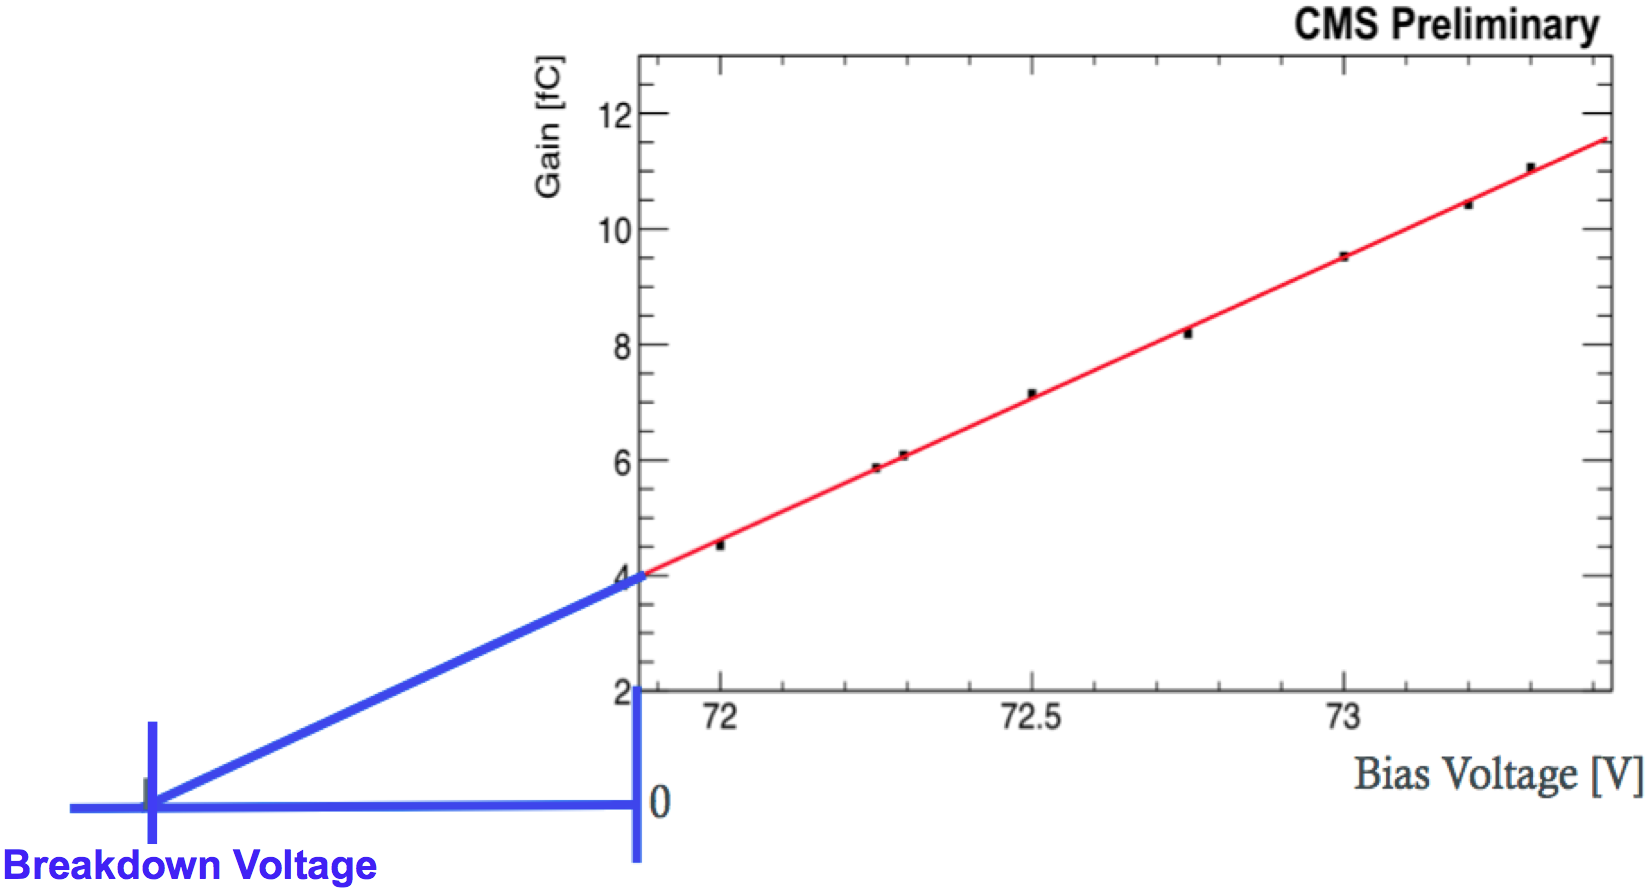
\includegraphics[width=0.9\textwidth]{Bilder/bvPedDetermination.png}
\caption{Determination of the breakdownvoltage of an SiPM using the gain from dark noise spectrums measured at different bias voltages.}
\label{bvPed}
%\end{minipage}
%\hspace{0.5cm}
\end{figure}
The determination of the breakdown voltage using the dark noise spectrum and the LED spectrum are shown in Fig. \ref{bvPed} and Fig. \ref{bvLed}, respectively.
\begin{figure}[h]
\centering
\begin{minipage}[t]{0.475\textwidth}
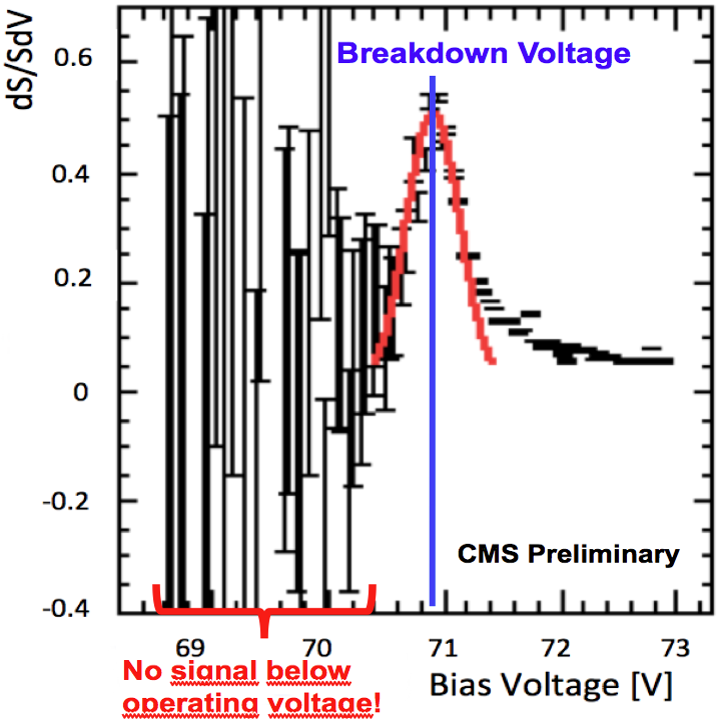
\includegraphics[width=\textwidth]{Bilder/bvLedScaled.png}
\caption{Breakdown voltage determination using the relative derivative of LED spectra measured at different bias voltages.}
\label{bvLed}
\end{minipage}
\hspace{0.5cm}
\begin{minipage}[t]{0.475\textwidth}

\end{minipage}
\end{figure}